\begin{frame}
	\frametitle{\lang,Figure placement,Figuurplaatsing,}

	\unless\ifishandout
	\only<1>{
		\hll|\\begin\{figure\}[h]|
		\smallskip

		\adjustbox{cfbox=black 1pt 0pt}{%
			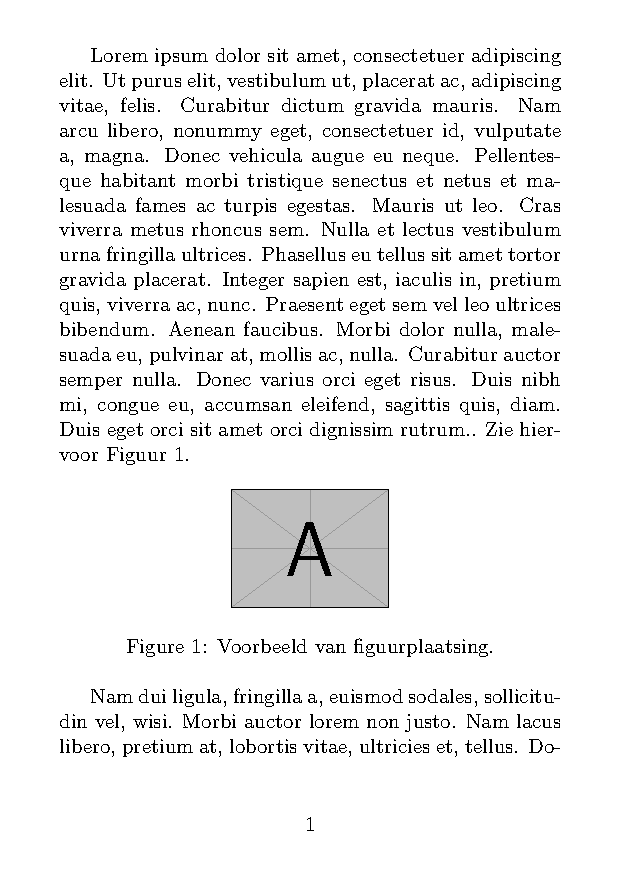
\includegraphics[
				page=1,width=0.4\textwidth,height=0.7\textheight,keepaspectratio
			]{assets/image_placement.pdf}
		}
		\adjustbox{cfbox=black 1pt 0pt}{%
			\includegraphics[
				page=2,width=0.4\textwidth,height=0.7\textheight,keepaspectratio
			]{assets/image_placement.pdf}
		}
	}
	\fi
	\only<2>{
		\hll|\\begin\{figure\}[t]|
		\smallskip

		\adjustbox{cfbox=black 1pt 0pt}{%
			\includegraphics[
				page=3,width=0.4\textwidth,height=0.7\textheight,keepaspectratio
			]{assets/image_placement.pdf}
		}
		\adjustbox{cfbox=black 1pt 0pt}{%
			\includegraphics[
				page=4,width=0.4\textwidth,height=0.7\textheight,keepaspectratio
			]{assets/image_placement.pdf}
		}
	}
	\unless\ifishandout
	\only<3>{
		\hll|\\begin\{figure\}[b]|
		\smallskip

		\adjustbox{cfbox=black 1pt 0pt}{%
			\includegraphics[
				page=5,width=0.4\textwidth,height=0.7\textheight,keepaspectratio
			]{assets/image_placement.pdf}
		}
		\adjustbox{cfbox=black 1pt 0pt}{%
			\includegraphics[
				page=6,width=0.4\textwidth,height=0.7\textheight,keepaspectratio
			]{assets/image_placement.pdf}
		}
	}
	\only<4>{
		\hll|\\begin\{figure\}[p]|
		\smallskip

		\adjustbox{cfbox=black 1pt 0pt}{%
			\includegraphics[
				page=7,width=0.4\textwidth,height=0.7\textheight,keepaspectratio
			]{assets/image_placement.pdf}
		}
		\adjustbox{cfbox=black 1pt 0pt}{%
			\includegraphics[
				page=8,width=0.4\textwidth,height=0.7\textheight,keepaspectratio
			]{assets/image_placement.pdf}
		}
	}
	\fi
\end{frame}

\addtorecentlist{htbp}

\begin{frame}
	\frametitle{\lang,Figure placement,Figuurplaatsing,}

	% Een figuur wordt ergens verderop geplaatst. Soms is het dus handig om een figuur
	% een paragraaf of twee the plaatsen voor de plek waar je hem gebruikt!
	
	\begin{itemize}
		\item h \textsc{(here)}: \lang,Figure can come here.,Figuur mag hier.,
		\item t \textsc{(top)}: \lang,Figure can come at the top of the page.,%
			Figuur mag bovenaan een pagina.,
		\item b \textsc{(bottom)}: \lang,Figure can come at the bottom of the
			page,Figuur mag onderaan een pagina.,
		\item p \textsc{(page)}: \lang,Figure can come on a special page for figures.,%
			Figuur mag op aparte pagina voor figuren.,
		\item !: \lang,Override internal parameters for floats.,Override interne parameters voor floats.,
		\item H \textsc{(here)}: \lang{No floating, always here.}
		{Geen floating, altijd hier.} (\hll|\\usepackage\{float\}|)
	\end{itemize}

	\medskip
	% \lang
	% {Figure appearing too late? Try placing \hll|figure| to a point earlier in the code.}
	% {Te laat in output? Verplaats \hll|figure| naar voren in je bestand.}

	\uncover<1->{\lang,When working with images,Wanneer je werkt met afbeeldingen,:
	\hll|\\usepackage\{graphicx\}|}
\end{frame}
